\documentclass[a4paper, 12pt]{article}
\usepackage[a4paper,top=1.5cm, bottom=1.5cm, left=1cm, right=1cm]{geometry}
\usepackage[utf8]{inputenc}
\usepackage{mathtext}
\usepackage{amsmath}
\usepackage{amsfonts}
\usepackage[english, russian]{babel}
\usepackage{indentfirst}
\usepackage{longtable}
\usepackage{graphicx}
\graphicspath{{pictures/}}
\DeclareGraphicsExtensions{.pdf,.png,.jpg}
\usepackage{natbib}
\usepackage{hyperref}
\usepackage{emoji}
\babelfont{rm}{Droid Serif}
\babelfont{sf}{Droid Sans}
\renewcommand{\baselinestretch}{1.3}

\title{1.3.2. Определение модуля кручения}
\author{Платонов Егор Б04-301}
\date{\today}

\begin{document}
	\maketitle
		\textbf{Цель работы:}Измерение углов закручивания в зависимости от приложенного момента сил, расчёт модулей кручения и сдвига при статическом закручивании стержня, определение тех же модулей для проволоки по измерениям периодов крутильных колебаний подвешенного на ней маятника(динамическим методом)
  
		\textbf{Оборудование:}В первой части: исследуемый стержень, отсчётная туба со шкалой, рулетка, микрометр, набор грузов;
		во второй части: проволока из исследуемого материала, грузы, секундомер, микрометр, линейка, рулетка.
	\section*{Теоретические сведения}
		При закручивании цилиндрических стержней круглого сечения распределение деформаций
 и напряжений одинаково по длине стержня только вдали от мест, где прикладываются закручивающие моменты.
Для этих областей можно считать, что каждое поперечное сечение поворачивается поворачивается как жествкое,
то есть частички материала не сходят с радиальных линий, на которых они были в начале, и все
эти линии поворачиваются на один и тот же угол. Такое напряженное состояние назвается чистым кручением.\\

При такой деформации любая прямая линия, проведенная до закручивания цилиндра почастицам материала и параллельная оси симметрии,
при закручивании превращается в спираль(винтовую линию). \\

Покажем, что касательное напряжение напряжение в поперечном сечении увеличивается пропорцианально
 расстоянию до оси вращения.
Рассмотрим в цилиндре колечко бесконечно малой толщиной $dr$ и высоты $dl$. При закручивании верхнее колечко поворачивается относительно 
нижнего на угол $d\varphi$, а образующая наклоняется на угол $\alpha$. Тогда при малы углах справедливо соотношение:
\begin{equation}
    \alpha dl= r d\varphi 
\end{equation}

Касательное наряжение $\tau $ связано с углом $\alpha$ линейной зависимостью через модуль сдвига $G$,
 и следовательно растет с увеличением расстоянием от оси:
\begin{equation}
    \tau = G\cdot \alpha =Gr\frac{d\varphi}{dl} 
\end{equation}

Эти касательные напряжения создают момент сил относительно оси цилиндра:

\begin{equation}
    dM=2\pi r dr \cdot r\cdot \tau  
\end{equation}

Интегрируя это выражение по всем колечкам от оси цилиндра до его радиуса R находим суммарный
момент сил:
\begin{equation}
    M = \frac{\pi G R^{4}}{2} \frac{d \varphi }{d l} 
\end{equation}

Так как момент сил не меняется по длине цилиндра. Тогда для связи приложенного
момента сил $M$ и угла поворота $\varphi$ поперечных сечений цилиндра имеем:
\begin{equation}
    M=\frac{\pi R^{4}G}{2l}\varphi=f \varphi
\end{equation}
Где $f$ - модуль кручения связанный с модулем сдвига $G$ соотношением:
\begin{equation}
    G=\frac{2l}{\pi R^{4}}f
\end{equation}

В системе можно возбудить крутильные колебания. Вращение стержня с закрепленными
на нем грузиками вокрунг вертикальной оси проиходит под действием упругого момента $M$.
С учетом выражения для момента $M$ получим, что это вращение описывается уравнением колебаний:
\begin{equation}
    I\frac{d^2 \varphi }{d t^2} + f \varphi =0
\end{equation}
Следовательно период кoлебаний системы связан с расстоянием $l$ от оси вращения до грузов и
моментом инерции стержня $I_0$ следующим образом:
\begin{equation}
    T^2=(2\pi)^2\frac{I}{f}=(2\pi)^2\frac{I_0}{f}+(2\pi)^2\frac{(m_1+m_2)}{f}l^2
\end{equation}
Эти зависимости были получены для незатухающих колебаний. Поэтому для их применения необходимо убедиться,
что в рассматриваемой системе диссипативными силами можно пренебречь. Для этого стоит убедиться, что период колебаний
не зависит от начальной амплитуды и что амплитуда уменшьется не более чем в 2 раза после около 10 колебаний.
\section{Определение модуля кручения статическим методом}
\subsection{Экспериментальная установка}
\begin{figure}[h]
    \centering
    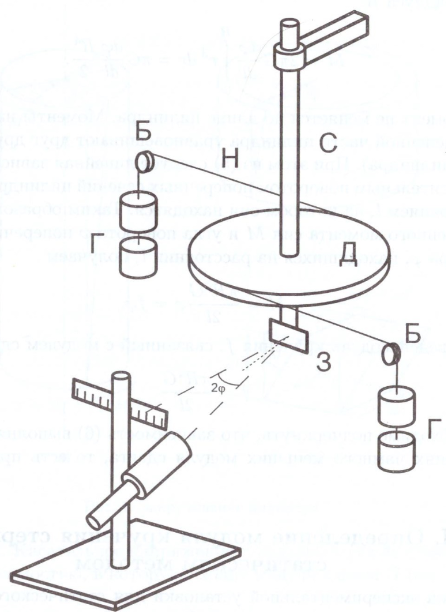
\includegraphics{stat.png}
    \caption{Схема установки}
    \label{fig:enter-label}
\end{figure}

Эту часть работы будем проводить на установке, схематично изображённой на рис. 1. Она состоит из вертикально расположенного стержня С, верхний конец которого прочно закреплён на стойке, а нижний соединён с диском Д. Момент $M$, закручивающий стержень создают две навитые на диск и перекинутые через блоки Б нити, к концам которых подвешиваются одинаковые грузы Г. Диск снабжён зеркальцем З. Для того, чтобы узнать угол поворота диска, нужно направить зрительную трубу на зеркальце и сделать так, чтобы в неё была чётко видна шкала, укреплённая на том же штативе, что и трубка. По изменению положения шкалы можно определить угол закручивания $\varphi$.
\subsection{Измерения и обработка результатов}
Расстояние от лазера до линейки $h = 152,2\pm0,1$ \text{см }($\varepsilon_h = 0,07\%$)

Диаметр диска $D = 10,7\pm0,05$ \text{см }($\varepsilon_D = 0,47\%$)

Радиус диска $R = \frac{D}{2} = 5,35 \pm0,025$ \text{см }($\varepsilon_R = 0,47\%$)

В таблице 1 представлена зависимость угла поворота стержня от момента приложенных к нему сил (6 серий измерений). Масса m в таблице, это масса груза, подвешеного на одну нить. На другую нить повешена такая же нагрузка.$\varphi = \arctg(\frac{x}{h})$, $M = 2mgR$. По этим же данным построен график зависимости $\varphi(M)$, изображенный на рисунке 2.

\begin{table}[h!]
 \centering
    \parbox{.4 \textwidth}{
        \centering
        \begin{tabular}{|l|l|l|l|}
        \hline
            $m$, г & $M$, Н$\cdot$м & $x \pm 0,05$ см & $\varphi$, рад \\ \hline
            100 & 0,105 & 2,9 & 0,019 \\ \hline
            150 & 0,157 & 5,2 & 0,034 \\ \hline
            200 & 0,21 & 8,4 & 0,055 \\ \hline
            250 & 0,262 & 10,3 & 0,067 \\ \hline
            350 & 0,367 & 16,7 & 0,109 \\ \hline
            450 & 0,472 & 21 & 0,137 \\ \hline
        \end{tabular}
        \label{tab:1}
    }
    \hfill
    \parbox{.5 \textwidth}{
        \centering
        \begin{tabular}{|l|l|l|l|}
        \hline
            $m$, г & $M$, Н$\cdot$м & $x \pm 0,05$ см & $\varphi$, рад \\ \hline
            100 & 0,105 & 2,5 & 0,016 \\ \hline
            150 & 0,157 & 5,7 & 0,037 \\ \hline
            200 & 0,21 & 7,8 & 0,051 \\ \hline
            250 & 0,262 & 10,5 & 0,069 \\ \hline
            350 & 0,367 & 15,8 & 0,103 \\ \hline
            450 & 0,472 & 21 & 0,137 \\ \hline
        \end{tabular}
        \label{tab:2}
    }
 \end{table}

 \begin{table}[h!]
 \centering
    \parbox{.4 \textwidth}{
        \centering
        \begin{tabular}{|l|l|l|l|}
        \hline
            $m$, г & $M$, Н$\cdot$м & $x \pm 0,05$ см & $\varphi$, рад \\ \hline
            100 & 0,105 & 2,6 & 0,017 \\ \hline
            150 & 0,157 & 5,7 & 0,037 \\ \hline
            200 & 0,21 & 8 & 0,053 \\ \hline
            250 & 0,262 & 10,5 & 0,069 \\ \hline
            350 & 0,367 & 16,1 & 0,105 \\ \hline
            450 & 0,472 & 20,5 & 0,134 \\ \hline
        \end{tabular}
        \label{tab:1}
    }
    \hfill
    \parbox{.5 \textwidth}{
        \centering
        \begin{tabular}{|l|l|l|l|}
        \hline
            $m$, г & $M$, Н$\cdot$м & $x \pm 0,05$ см & $\varphi$, рад \\ \hline
            100 & 0,105 & 2,5 & 0,016 \\ \hline
            150 & 0,157 & 5,4 & 0,035 \\ \hline
            200 & 0,21 & 7,8 & 0,051 \\ \hline
            250 & 0,262 & 10,8 & 0,071 \\ \hline
            350 & 0,367 & 16 & 0,105 \\ \hline
            450 & 0,472 & 20,5 & 0,134 \\ \hline
        \end{tabular}
        \label{tab:2}
    }
 \end{table}

  \begin{table}[h!]
 \centering
    \parbox{.4 \textwidth}{
        \centering
        \begin{tabular}{|l|l|l|l|}
        \hline
            $m$, г & $M$, Н$\cdot$м & $x \pm 0,05$ см & $\varphi$, рад \\ \hline
            100 & 0,105 & 2,6 & 0,017 \\ \hline
            150 & 0,157 & 5 & 0,033 \\ \hline
            200 & 0,21 & 8,2 & 0,054 \\ \hline
            250 & 0,262 & 10,2 & 0,067 \\ \hline
            350 & 0,367 & 15,9 & 0,104 \\ \hline
            450 & 0,472 & 21,5 & 0,14 \\ \hline
        \end{tabular}
        \label{tab:1}
    }
    \hfill
    \parbox{.5 \textwidth}{
        \centering
        \begin{tabular}{|l|l|l|l|}
        \hline
            $m$, г & $M$, Н$\cdot$м & $x \pm 0,05$ см & $\varphi$, рад \\ \hline
            100 & 0,105 & 2,7 & 0,018 \\ \hline
            150 & 0,157 & 5,2 & 0,034 \\ \hline
            200 & 0,21 & 8,1 & 0,053 \\ \hline
            250 & 0,262 & 10,9 & 0,071 \\ \hline
            350 & 0,367 & 16,1 & 0,105 \\ \hline
            450 & 0,472 & 21,5 & 0,14 \\ \hline
        \end{tabular}
        \label{tab:2}
    }
 \end{table}
 
 \begin{center}
     Таблица 1
 \end{center}

По МНК найден коэффициент наклона $k = 0,328 \frac{\text{рад}}{\text{Н$\cdot$м}}$. При подсчете систематической погрешности учтено, что относительные погрешности величин примерно одинаковые, в формуле используются значения, ближайшие к среднему ($\varepsilon_{\varphi} = 0,05 \%, \varepsilon_M = 0,05 \%$).

\[ \sigma_k^{\text{случ}} = \frac{1}{\sqrt{N - 2}}\sqrt{\frac{\langle \varphi^2 \rangle -\langle \varphi \rangle^2}{
    \langle M^2 \rangle - \langle M \rangle^2} - k^2}\]

\[ \sigma_k^{\text{сист}} = k\sqrt{(\varepsilon_{\varphi})^2+(\varepsilon_M)^2}\]

\[ \sigma_{k} = \sqrt{\sigma_k^{{\text{сист}}^2}+\sigma_k^{{\text{случ}}^2}} = 0,0037 \text{ }\frac{\text{рад}}{\text{Н$\cdot$м}}\]

\[ \varepsilon_k = \frac{\sigma_k}{k} = 1,13 \%\]

Из формулы (5) следует, что
\[f = \frac{1}{k} = 3,05 \text{ }\frac{\text{Н$\cdot$м}}{\text{рад}}\text{ }(\varepsilon_f = 1,13 \%)\]

Длина стержня $l = 1,33 \pm 0,001$ м ($\varepsilon_l = 0,07\%$)

Диаметр сечения стержня $d = 0,6 \pm 0,005$ см ($\varepsilon_d = 0,83\%$)

Радиус сечения стержня $r = 0,3 \pm 0,0025$ см ($\varepsilon_r = 0,83\%$)

Модуль сдвига G вычислен по формуле (6):
\[G = 31,88 \text{ ГПа}\]

\[ \varepsilon_G = \sqrt{\varepsilon_l^2+\varepsilon_f^2+(4\varepsilon_r)^2} = 3,5 \%\]

 \begin{figure}[h!]
     \centering
     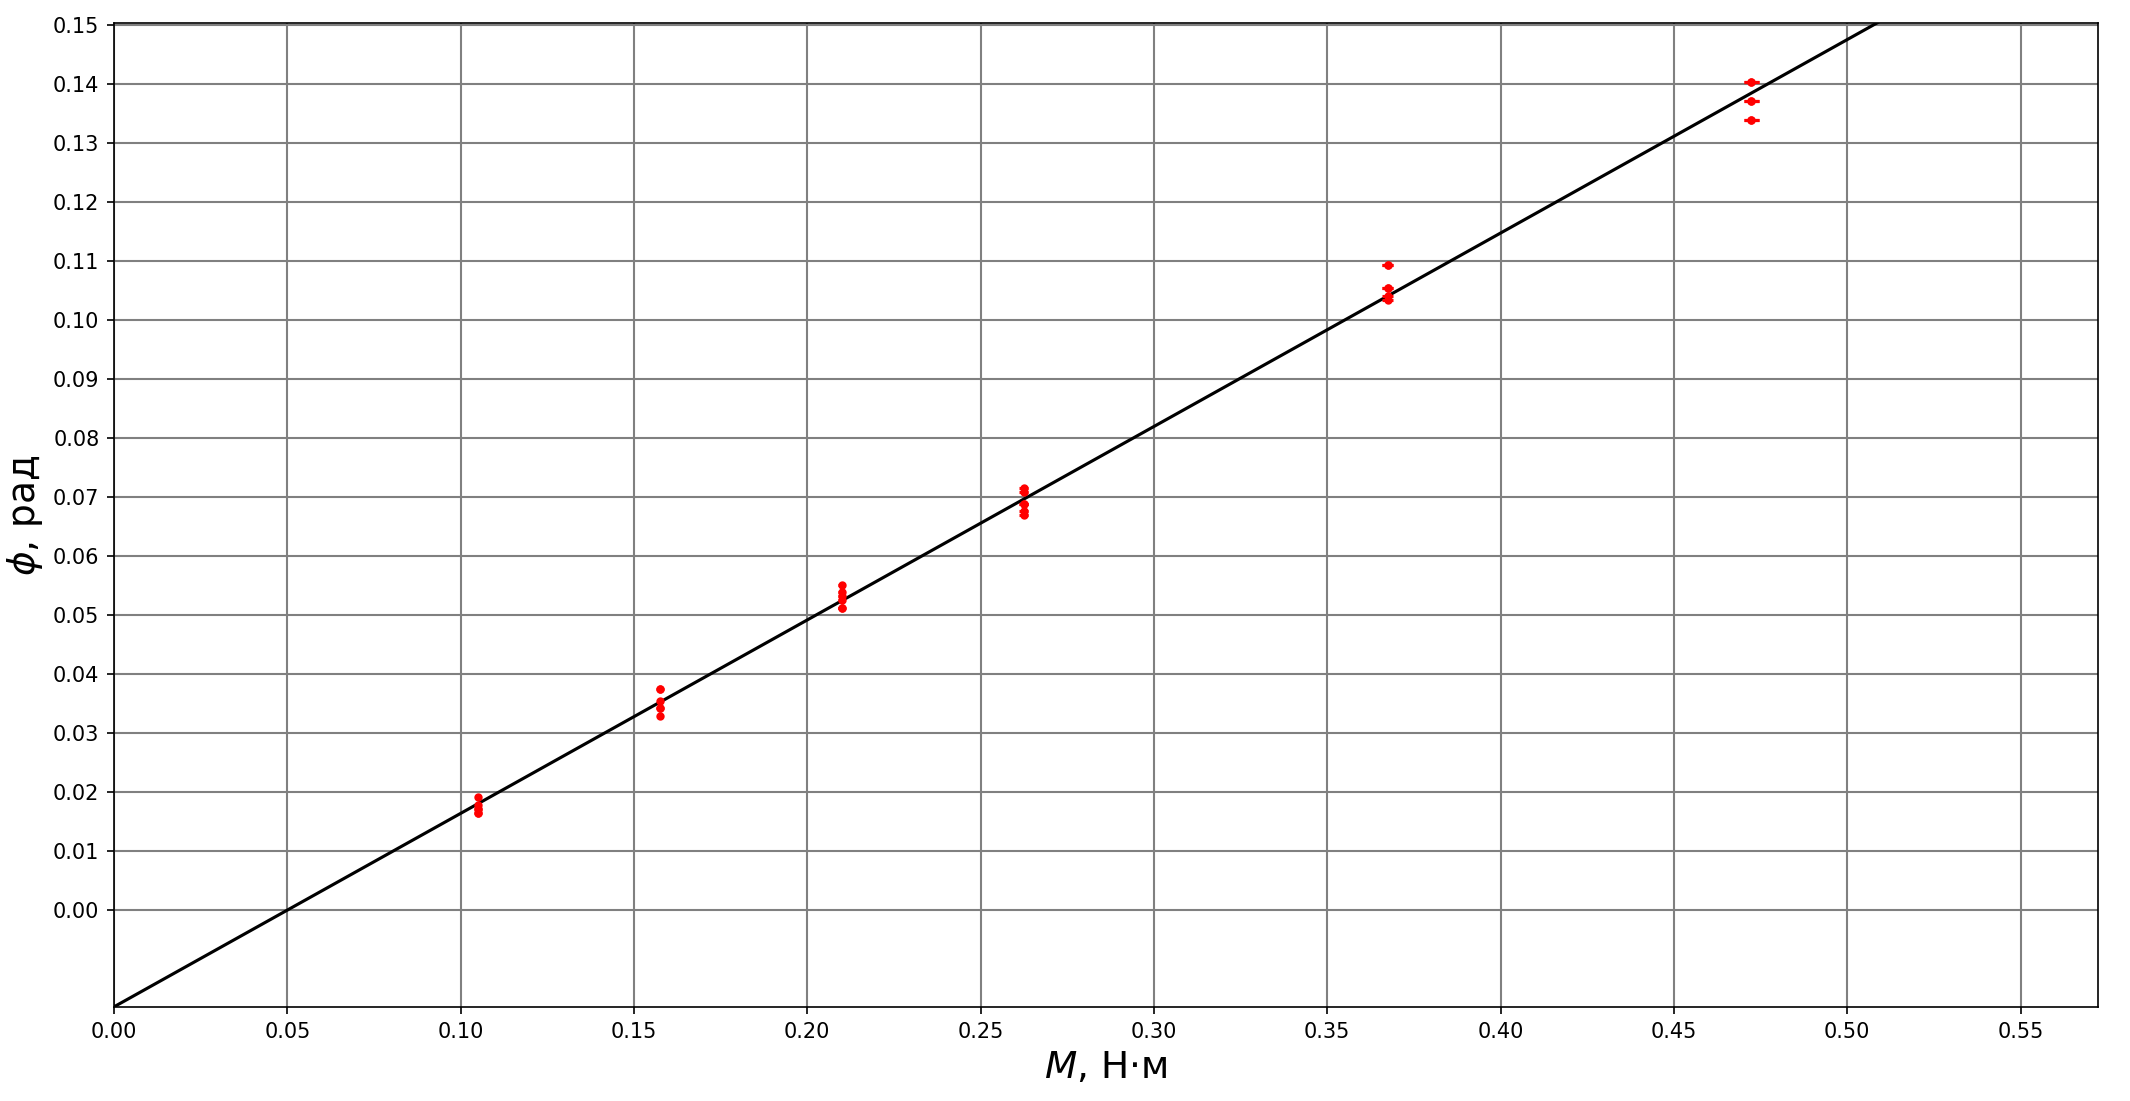
\includegraphics[scale = 0.5]{plota.png}
     \caption{Зависимость $\varphi(M)$}
     \label{fig:enter-label}
 \end{figure}


\section{Определение модуля кручения при помощи крутильных колебаний}
\subsection{Экспериментальная установка}
\begin{figure}[h]
    \centering
    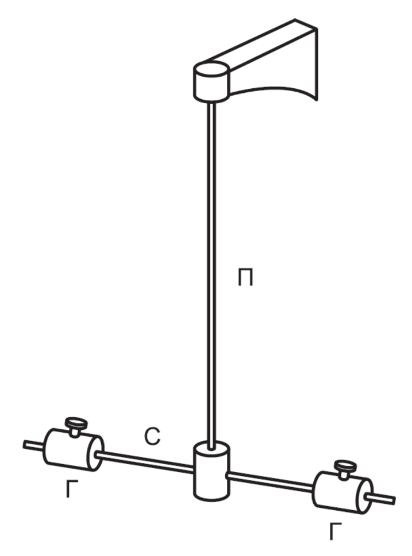
\includegraphics{dyn.png}
    \caption{Схема установки}
    \label{fig:enter-label}
\end{figure}
Экспериментальная установка, использующаяся на данном этапе работы состоит из длинной висячей проволоки П, к нижнему её концу прикреплён горизонтальный стержень С, на котором симметрично закреплены грузики Г. 
\subsection{Измерения и обработка результатов}
Зависимость периода колебаний от длины плеча (расстояние от оси вращения до грузиков) представлена в таблице 2.
\begin{table}[!ht]
    \centering
    \begin{tabular}{|l|l|}
    \hline
        $l \pm 0,05$ см & $T\pm 0,002$ с \\ \hline
        6,4 & 2,15 \\ \hline
        7,4 & 2,387 \\ \hline
        8,4 & 2,613 \\ \hline
        9,4 & 2,875 \\ \hline
        10,4 & 3,124 \\ \hline
        11,4 & 3,396 \\ \hline
    \end{tabular}
    \caption{Зависимость периода колебаний от длины плеча}
\end{table}
На рисунке 4 представлен график зависимости $l^2$($T^2$).
\begin{figure}[h]
    \centering
    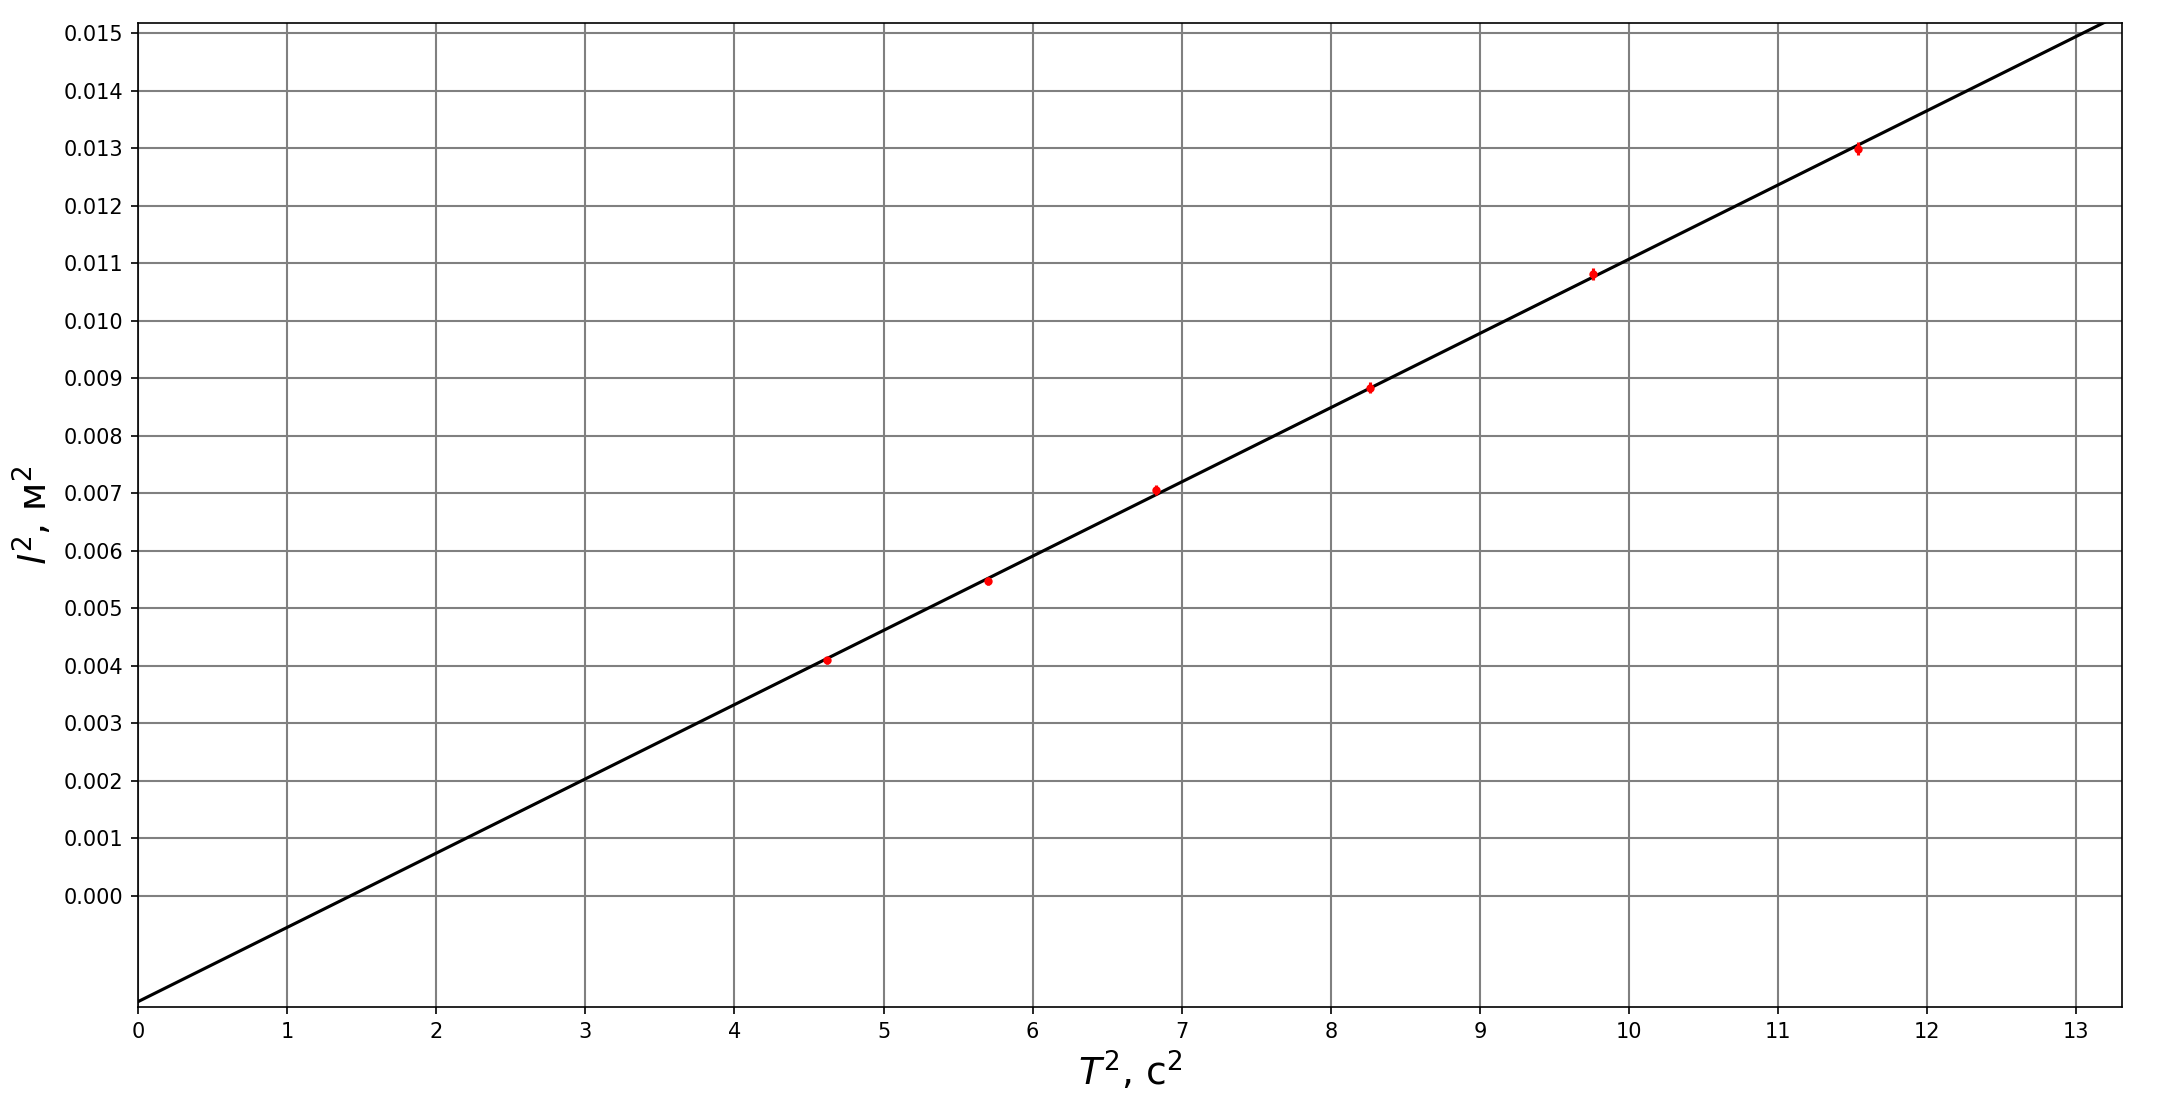
\includegraphics[scale = 0.5]{plotb.png}
    \caption{зависимость $l^2$($T^2$)}
    \label{fig:enter-label}
\end{figure}
По МНК найден коэффициент наклона $k = 0,0013 \frac{\text{м}^2}{\text{c}^2}$. При подсчете систематической погрешности учтено, что относительные погрешности величин примерно одинаковые, в формуле используются значения, ближайшее к среднему ($\varepsilon_l = 0,05 \%, \varepsilon_T = 0,07 \%$).

\[ \sigma_k^{\text{случ}} = \frac{1}{\sqrt{N - 2}}\sqrt{\frac{\langle {l}^4 \rangle -\langle {l^2} \rangle^2}{
    \langle T^4 \rangle - \langle T^2 \rangle^2} - k^2}\]

\[ \sigma_k^{\text{сист}} = k\sqrt{(2\varepsilon_l)^2+(2\varepsilon_T)^2}\]

\[ \sigma_{k} = \sqrt{\sigma_k^{{\text{сист}}^2}+\sigma_k^{{\text{случ}}^2}} = 0,0000175 \text{ }\frac{\text{м}^2}{\text{с}^2}\]

\[ \varepsilon_k = \frac{\sigma_k}{k} = 1,35 \%\]
$m_1 = (377,5 \pm 0,5)$ г, $m_2 = (373,1 \pm 0,5)$ г

$m = (750,6 \pm 1)$ г ($\varepsilon_m = 0,13 \%)$

Из формулы (8) следует, что
\[f=4\pi^2(m1+m2)*k = 0,0385 \frac{\text{Н}\cdot\text{м}}{\text{рад}}\]

\[ \varepsilon_f = \sqrt{\varepsilon_k^2+\varepsilon_m^2} = 1,36 \%\]

Длина проволоки $l = 1,75 \pm 0,002$ м ($\varepsilon_l = 0,11\%$)

Диаметр сечения проволоки $d = 1,98\pm 0,005 $ мм ($\varepsilon_d = 0,25\%$)

Радиус сечения проволоки $r = 0,99\pm 0,0025 $ мм ($\varepsilon_r = 0,25\%$)

Модуль сдвига G вычислен по формуле (6):
\[G = 44,65 \text{ ГПа}\]

\[ \varepsilon_G = \sqrt{\varepsilon_l^2+\varepsilon_f^2+(4\varepsilon_r)^2} = 1,7 \%\]

\section{Вывод}
В результате эксперимента были получены модуль кручения стержня $(3,05 \pm 0,03) \text{ }\frac{\text{Н$\cdot$м}}{\text{рад}}\text{ }(\varepsilon_f = 1,13 \%)$ и его модуль сдвига $G = (31,88 \pm 1,12) \text{ ГПа} (\varepsilon_G = 3,5 \%)$, что находится рядом со значениями модуля сдвига для меди, бронзы, латуни и серебра.

Также были найдены модуль кручения проволоки $(0,0385 \pm 0,0005) \text{ }\frac{\text{Н$\cdot$м}}{\text{рад}}\text{ }(\varepsilon_f = 1,36 \%)$ и её модуль сдвига $G = (44,65 \pm 0,76) \text{ ГПа} (\varepsilon_G = 1,7 \%)$, что находится рядом со значением модуля сдвига для меди.

\end{document}
